\chapter{Literature Review}
\label{Literature Review}

This chapter reviews the literature pertinent to this research topic. It covers the development of bearing models, ranging from simple quasi-static to high-degree-of-freedom (DOF) dynamic models. Recent advancements on the implicit coupling of tribological and dynamic bearing models is then reviewed. The fundamentals of contact mechanics, essential to the research questions, are introduced alongside a discussion of contact modelling techniques. An overview of elastohydrodynamic lubrication modelling, including numerical methods, characteristics, regimes of lubrication and empirical formulae is presented. Finally, the application of artificial neural networks in the field of tribology and their impact on future modelling is explored.

\section{Rolling Element Bearing Introduction}

The term rolling element bearing encompasses both ball and roller type bearings. These common machine elements permit motion of, or about, shafts in a wide range of devices; from wheel bearings in bicycles and cars to electric motors and aircraft gas turbines. In automotive transmissions, these bearings support the rotation of the shaft and the radial and axial forces applied during gear meshing. Single or two stage gearing in electric transmissions mean that bearings in both the electric motors and input shaft to the gearboxes operate under high speeds, in excess of 32~000~$rpm$.

The general use of rolling element bearings occurred from the start of the Industrial Revolution, however the origin of what constitutes modern bearing design dates back as far as $ca.$1500. Leonardo Da Vinci, in his Codex Madrid, conceived a thrust ball bearing design consisting of spherical balls with conical separation elements \cite{Harris2007}.

Prior to the scientific advancements of the atomic age, the design of rolling element bearings was regarded as more an art than a science. Alas, this thesis is not a work of art (hyberbole notwithstanding), but rather an advancement of the scientific knowledge that precedes it.

\section{Rolling Element Bearing Modelling}

Before the 1960’s, bearing studies were primarily conducted experimentally. Empirical formulations were derived to model their performance in early work by Stribeck \cite{Stribeck1907} and Lundberg and Palmgren \cite{Lundberg1952} \cite{Palmgren1959} amongst others. As computer technology improved post-1960, modelling theory and application grew rapidly, pioneered largely by the work of Jones \cite{Jones1960} and Harris \cite{Harris1984}. In the pursuit of highly efficient and reliable bearings, modelling and the need for accurate representation of the physical phenomena has become important. It is not possible to conduct experimental testing for the large array of design and operational parameters that bearings are required for, therefore experimentally validated numerical analysis is employed.

\subsection{Quasi-static Bearing Models}

Early models predicting load distribution in the rolling elements can calculate bearing stiffness and fatigue life with relative accuracy. These were primarily quasi-static and based on force equilibrium. Studies of static ball bearings under simple radial loading were performed by Stribeck \cite{Stribeck1907} and improved upon by Palmgren \cite{Palmgren1959} for the case of nominal internal clearance. Static models computing radial and axial loads based on a load distribution factor and the angular position of the roller were found using Sjovall’s integration model \cite{Sjovall1933}, however this was only applicable if the ratio of radial to axial loads is within a particular range. Rumbarger \cite{JRumbarger1962} developed a model using Sjovall’s integral method for purely axial loading of thrust bearings, capable of calculating moment load due to axial load eccentricity. 

It was the work of Jones \cite{Jones1960} and his general theory for load deflection analysis of bearings that extended the capability of these models. His work accounted for centrifugal and gyroscopic loading, and unlike previous models, the inner bearing race had 5 degrees of freedom (DOFs); three translational and two rotational displacements that correspond to the external forces in all three cartesian coordinates and moments applied about two. Bearing equilibrium is obtained at each rolling element by observing the load and corresponding motion of the elements. Jones also included the individual stiffness at the contact between rolling elements and raceways, using the Hertzian contact load-deflection relationship to obtain roller load based on contact deflection. This technique could be applied to both ball and roller bearings by varying the exponent of localised deflection. 

Jones' model was considerd limited due to the assumption that misalignment effects on the elements are negligible. Harris \cite{Harris1984} improved on it by introducing the slicing method along the length of the rollers. This enabled determination of the load distribution along the contact in roller bearings. This method, known as the Jones-Harris method, was then applicable for highly loaded conditions and able to compute misaligned cases. Vector and matrix methods to analytically solves the quasi-static problem based on the work of Jones and Harris were then presented for tapered roller bearing cases by Andréason \cite{Andreason1973} and Liu \cite{Liu1976}. de Mul et al. \cite{DeMul1989_2} developed a model for ball and roller bearing equilibrium and stiffness matrix calculations which has the advantage of having load-deflection equations in matrix form, therefore implementation of this model is simpler.

Additional functionality has been added to these models such as the effects of thermal expansion on the load-deflection analysis \cite{Jorgensen1997}. Numerical models for heat generation based on frictional torque and 3-dimensional transfer through contacting elements was used to account for the expansion. It was found that expansion increased the bearing stiffness and thus natural frequency of the shaft-spindle system due to greater interference of the roller race contact. The authors also investigated the effect of ring expansion due to centrifugal force at high speeds \cite{Jorgensen1998} and found that natural frequency of the spindle decreased at higher rotational speeds – of particular note for high speed automotive applications.

Quasi-static models are only applicable under steady-state operating conditions; however, the static equilibrium solutions \cite{Andreason1973} \cite{Liu1976} \cite{DeMul1989_1} are of use to calculate load-deflection and individual element loading within dynamic models.

\subsection{Dynamic Bearing Models}
Transient operating conditions such as acceleration or deceleration of the bearing requires dynamic modelling, particularly important for high-speed applications. In dynamic bearing models, a system of differential equations based on Newton’s second law of motion are used. This allows for a time-varying input force such as eccentric rotor unbalances or fluctuating loading conditions present in transmissions. Static equilibrium solutions such as those presented are used within these models to calculate load-deflection and individual element loading. 

Hitherto, a multitude of models predicting bearing dynamics have been posed for roller bearings. These investigate the dynamic effect of geometrical and topographical parameters such as surface waviness, surface defects, and the variable compliance affect. This variable compliance effect is caused by time-varying stiffness variations off the inner and outer race bearing contact as rollers change their orbital position and pass through the loaded region. Even with perfect bearing geometry free from any defects, vibration will still occur due to this \cite{Sopanen2003_1}.
  
Simplified 2 degree of freedom models \cite{Walters1971} consider purely in-plane motion of rolling elements in the radial and lateral directions of the bearings for investigation of frequency response to defects \cite{Meyer1980} and the varying compliance effect \cite{Sunnersjo1978}.  Time varying forces on cutting tool spindles and the effects on radial loading assuming no axial thrust loads or vibration can also be investigated in 2 DOF \cite{Matsubara1988}. These models increase in complexity up to 5-DOF  to observe moment loading and centrifugal effects \cite{Gupta1979} \cite{Aini1990} \cite{Rahnejat2004}. Most of these models assume the bearing rollers and races are rigid bodies. All of these analyses also assume a dry contact between rolling elements and races which was assumed valid under the elastohydrodynamic regime of lubrication. The fluid film behaves as an amorphous, incompressible solid and generated pressures conform closely to a Hertzian distribution in the loaded region. This, however, neglects the effect of the lubricant film thickness in the contact mechanics and thus underestimates the contact deflection and hence load.

\subsection{Lubricated Dynamic Bearing Models}

Based on the experimental and numerical findings \cite{Questa2020} \cite{Stone1982} \cite{Dietl1997}, the EHL film at the roller-race conjunction can be shown to increase the bearing stiffness, which continues to rise non-linearly with speed. It is therefore clear that the lubricant film in roller bearings operating at high speeds must be implicitly included in dynamic analyses. As stated by Bizarre et al. \cite{Bizarre2018}, there are few studies in the open literature that combine the stiffness and damping of an EHL contact with classical bearing dynamics.

Historically the analysis of rolling element bearings has been decoupled into two stages. The first stage is a classic dry Hertzian-contact analysis of the roller-raceway contact due to the cyclic variation in geometric bearing centre.  The displacement of the bearing centre is obtained through solving equations of motion and roller load is obtained using the Hertzian load-deflection relationship. Extrapolated film thickness equations use the transient load yielded from dry analysis in a second stage study to find central film thickness. This approach does not implicitly consider the effect of the lubricant film on the prevailing bearing motion and load, which is hence underestimated. To overcome these shortcomings, quasi-static analyses employing film thickness formulae in conjunction with Hertzian contact mechanics are required.

Early lubricated bearing models use extrapolated formulae to provide a relationship between the load share and film thickness at each element’s contact with the bearing raceways \cite{Rahnejat1985}. Aini et al. \cite{Aini2002} implemented the extrapolated film approach from the work of Rahnejat and Gohar \cite{Rahnejat1985} into a five-DOF bearing equilibrium model. The work computes the deformation at each roller–race contact, combining the EHL film thickness with the elastic deformation of the contacting solids. The force–displacement relationship is shown to follow a non-linear trend.

Film shape and the elastohydrodynamic pressure profile at the contact could not be calculated in these studies, preventing more detailed analysis such as thermal and sub-surface stress analysis. To determine tribological contact conditions, Mohammadpour et al. \cite{Mohammadpour2015c} employed a similar implicit tribodynamic analysis and then utilised a full numerical EHL analysis explicitly for further tribological studies.

Mohammadpour et al. \cite{Mohammadpour2015c} employed a similar implicit tribodynamic analysis and then utilised a full numerical EHL analysis explicitly for further tribological studies. In their analysis, input shaft speeds of 209~$rad/s$ resulted in much slower entrainment velocities than are applicable for electrified powertrain analyses. 

Film shape and the elastohydrodynamic pressure profile at the contact could not be calculated in these studies, preventing more detailed analysis such as thermal and sub-surface stress analysis. To determine tribological contact conditions, Mohammadpour et al. \cite{Mohammadpour2015c} utilised a full numerical elastohydrodynamic analysis explicitly. Load values on an individual roller at each instantaneous position of the orbit were obtained from the implicit tribodynamic analysis and used within the numerical model.

Sopanen and Mikkola \cite{Sopanen2003_1} modelled the influence of various surface characteristics on bearing dynamics, including contributions from surface waviness, roughness, localised and distributed effects. Their six-DOF model accounts for the Hertzian contact deformation and the EHL film implicitly within the contact. This model was embedded in a multi-body dynamic (MBD) software to utilise its mathematical capabilities. This work does not, however, demonstrate the effect that the EHL film has on bearing stiffness, and the effect on system dynamics using flexible bodies is not analysed \cite{Sopanen2003_2}. Sawalhi and Randall \cite{Sawalhi2008} used a constant preload approach to imitate the stiffening effect of the film. Whilst this effective preload captures the increased contact stiffness due to the presence of the EHL film, the film thickness does not vary based on the contact conditions.

More recently, Liu and Shao \cite{Liu2017b} investigated the effects of surface waviness, including the effect of the lubricant film using an equivalent stiffness model. Nonato and Cavalca \cite{Nonato2014} presented a methodology to model EHL contacts using a set of non-linear springs and viscous dampers. Bizarre et al. \cite{Bizarre2018} applied this lubricated non-linear force contact to a five-DOF model of an angular contact ball bearing. This enabled a combined solution scheme for the bearing force equilibrium and the EHL contact. The formulated system of equations was solved, achieving force equilibrium for each rotation of a bearing under constant external load. The authors of this study noted the interest of combining such models within FMBD system level models.

None of the combined models above are embedded within a system level model comprising flexible bodies, and the effect of the change in the contact stiffness due to the lubricant film is not investigated at the system level. Furthermore, the high-speed operation and time-varying loads representative of electrified vehicle transmissions are not considered.

\section{Contact Mechanics}
A critical aspect of this work is the interface between rolling element and race; a field of engineering referred to as Contact Mechanics. The following section gives a brief introduction to the modelling and development of such models. This subject is elaborated further in Section \ref{Contact mechanics experimental tribodynamics} and Section \ref{Contact mechanics FMBD}.

\subsection{Hertzian Contact Mechanics}

Two types of contacts occur in machine elements: conformal and non-conformal. Conformal contacts occur between a concave and a convex body of similar radius, such as in journal bearings. This leads to a relatively large contact area over which load can be distributed and resultant pressures are in the order of $MPa$. The contact between rolling elements and races is non-conformal in nature as the contacting surfaces are both convex. This type of contact creates a very small contact region over which force is transmitted, leading to very high contact pressures being generated in the order of $GPa$. Under these pressures, the contact surfaces deform elastically. In the case of a lubricated contact, a lubricant film forms in between the contacting surfaces in the order of microns (typically < 2~$\mu \mathrm{m}$) \cite{Gohar2018}. Non-conformal contacts are typically found in rolling element bearings, gear contacts and cam follower pairs.

A fundamental characteristic of these contacts is that the approach of the bodies under external load leads to the deformation of both bodies and the emergence of a contact patch. For two cylinders in contact with their axes parallel, a rectangular or line contact is formed along the length of the cylinders with width $2b$ (see Figure \ref{LineContact}). An elliptical point contact results from contacting bodies that have different radii along both principal axes \cite{Johnson1985} (see Figure \ref{PointContact}). In the case of cylindrical elements, such as those in Needle Roller Bearings (NRBs), Cyclindrical Roller Bearings (CRBs) and Tapered Roller Bearings (TRBs), the mutual approach of the roller and race forms a line contact. Spherical elements, such as those found in Deep Groove Ball Bearings (DGBBs) and Angular Contact Ball Bearings (ACBBs), generate an elliptical contact at their conjunction with the raceway.

\begin{figure}
	\centerline{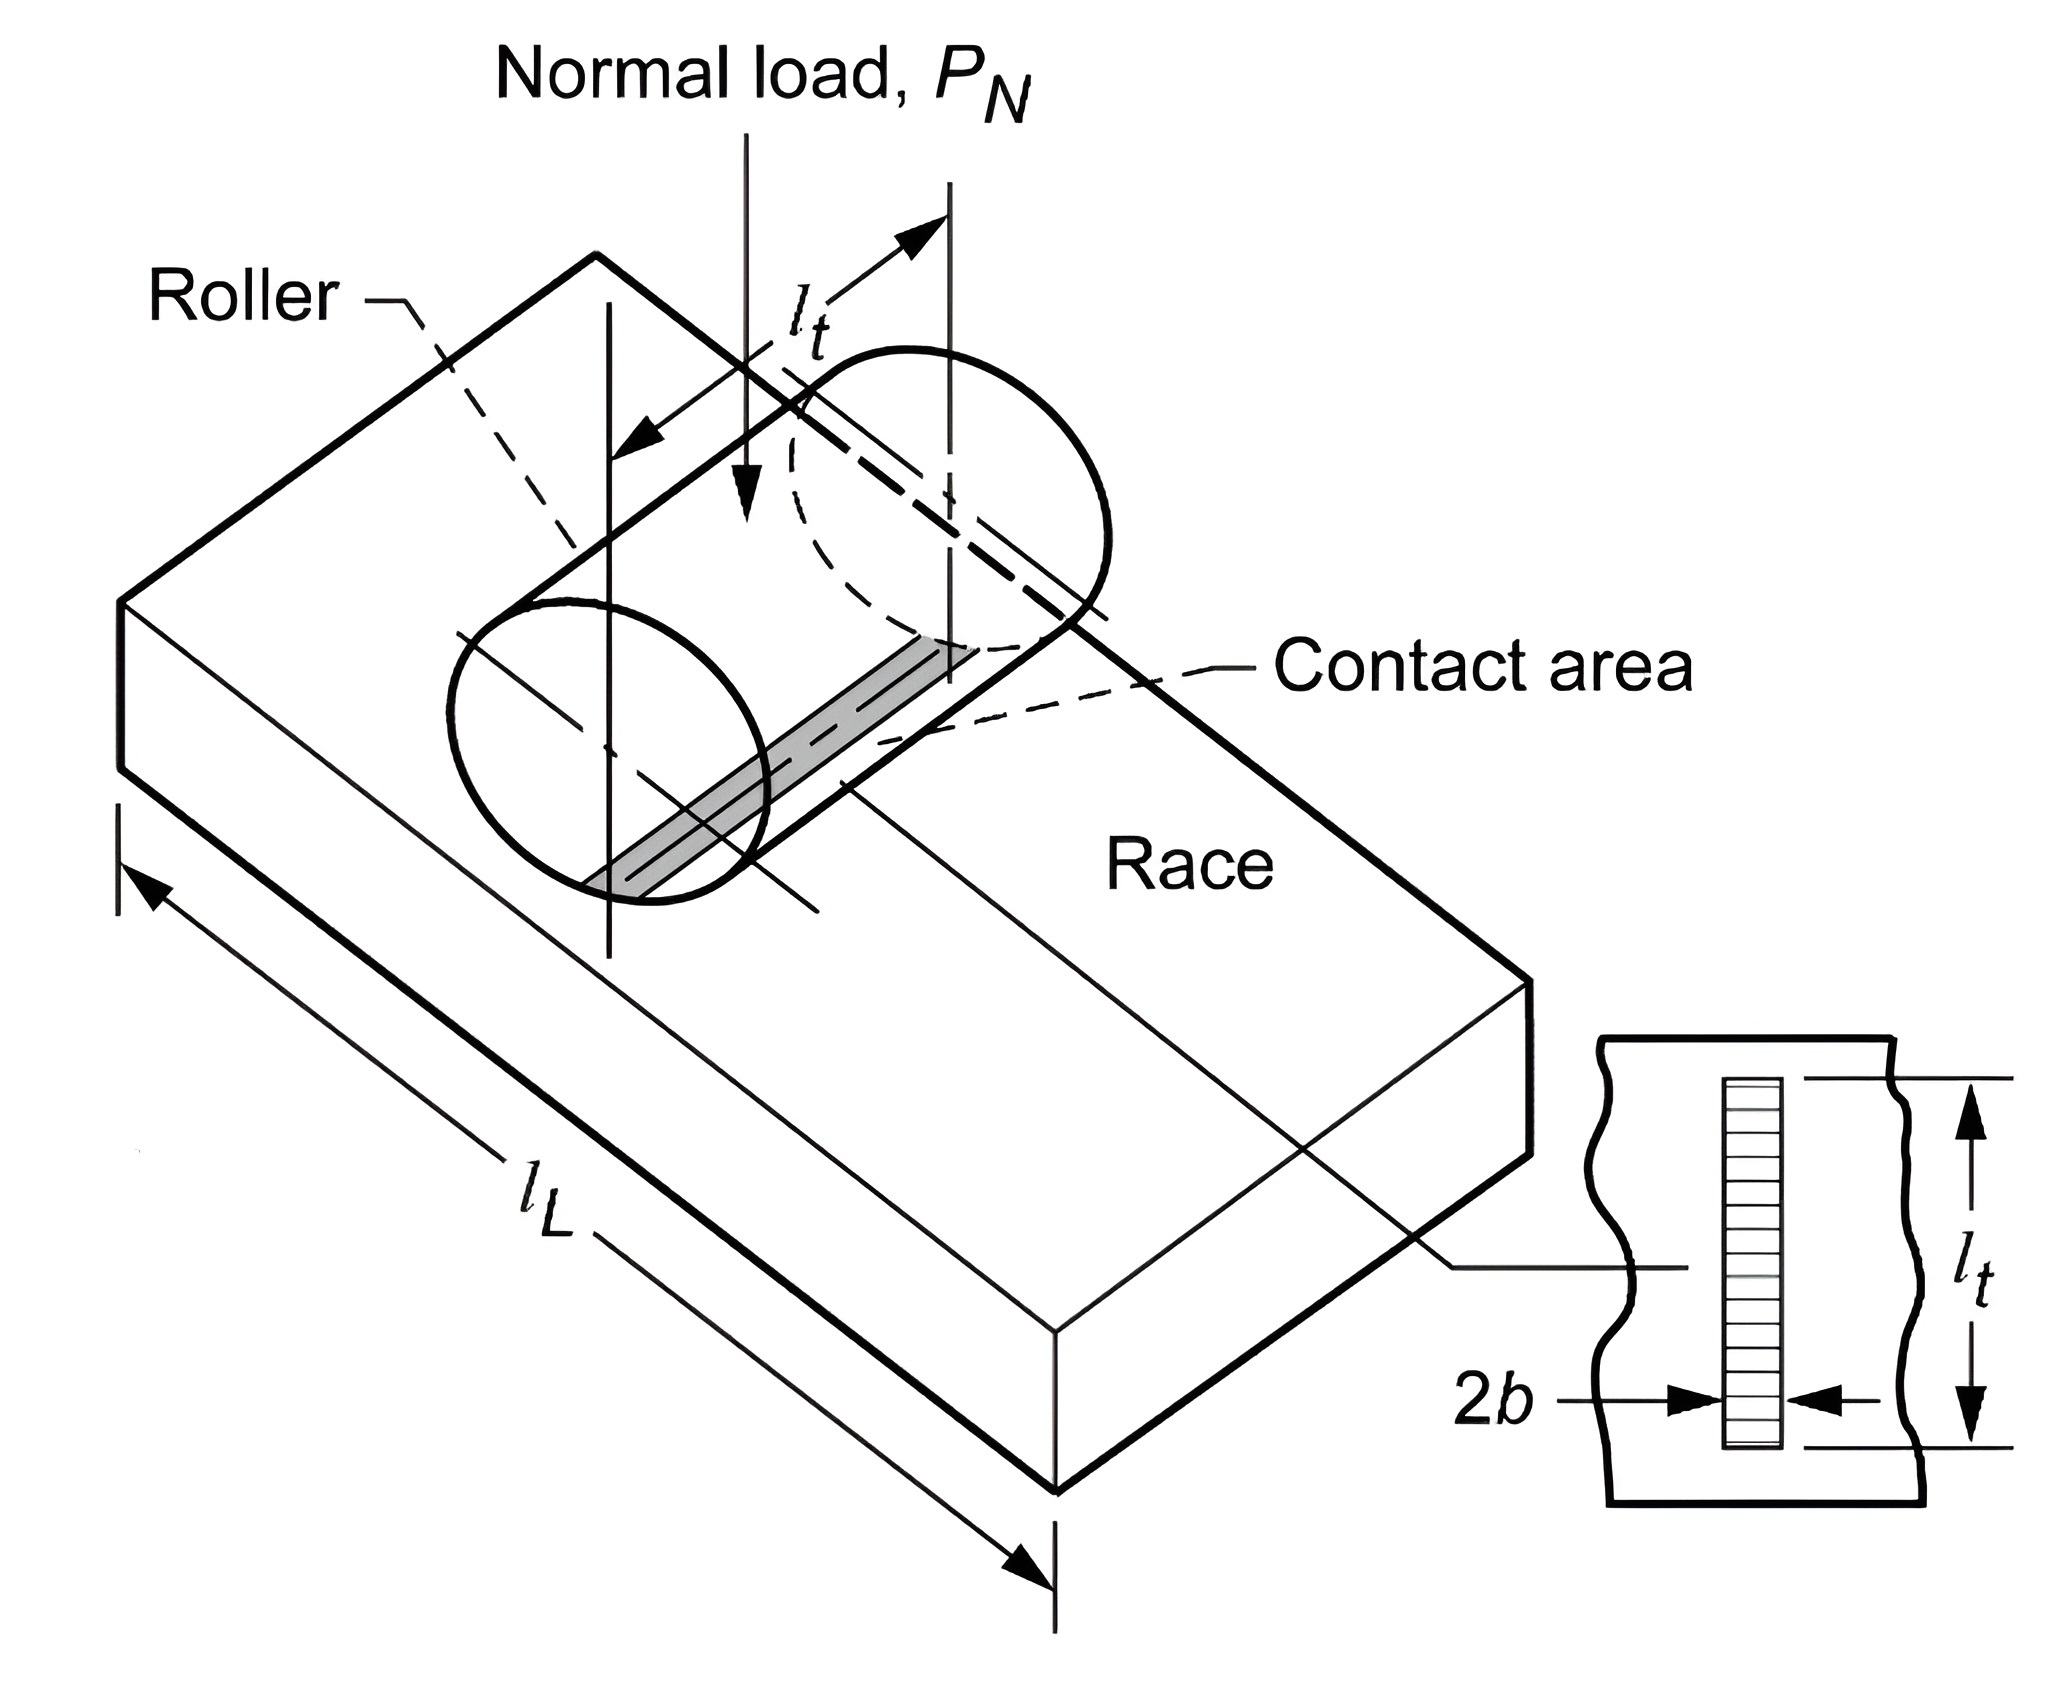
\includegraphics[width=110 mm]{LineContact.png}}
	\caption[Roller-race model for line contact]{Roller-race model for line contact \cite{Zaretsky2016}.}
	\label{LineContact}
\end{figure}

\begin{figure}
	\centerline{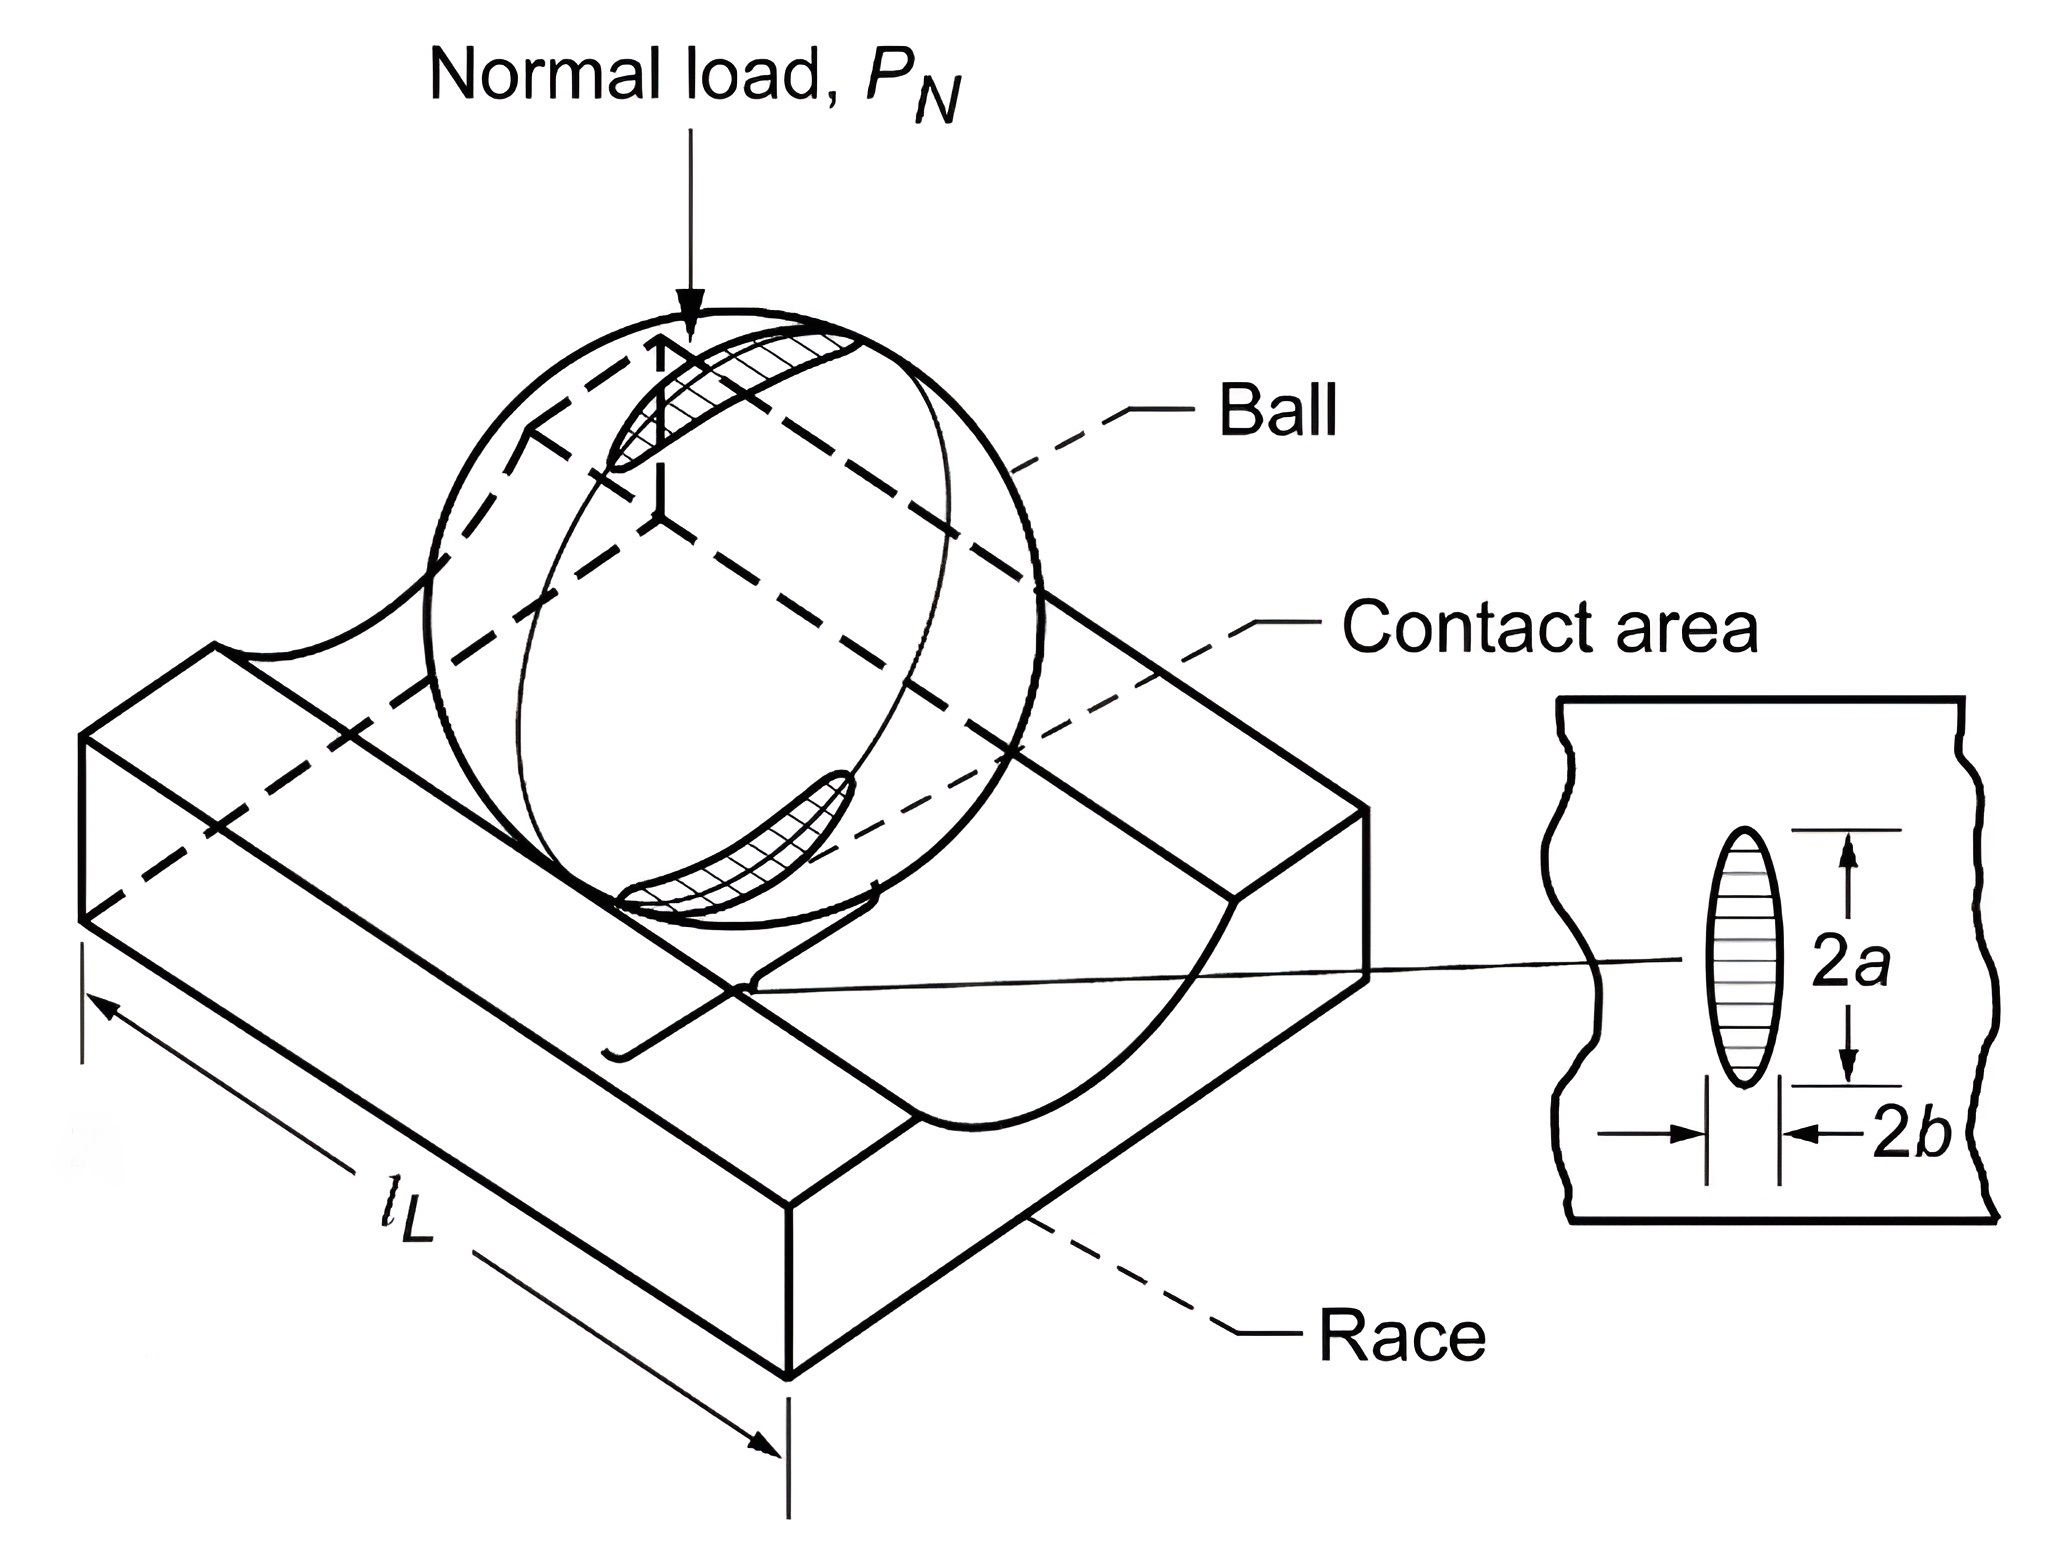
\includegraphics[width=110 mm]{PointContact.png}}
	\caption[Ball-race model for point contact]{Ball-race model for point contact \cite{Zaretsky2016}.}
	\label{PointContact}
\end{figure}

Two cylinders with radii $R_1$ and $R_2$ contacting in a non-conformal manner can be simplified as a rigid cylinder in contact with an elastic half-space. This cylinder, as represented in Figure \ref{LineContact}, has a radius known as the reduced radius, $R^{\prime}$:

\begin{equation}\label{eq2.1}
	\frac{1}{R^{\prime}}=\frac{1}{R_1}+\frac{1}{R_2}
\end{equation}

The material properties of the two bodies are evaluated in a similar way. The elastic modulus, $E$ and Poisson's ratio, $v$, of both bodies are combined to calculate the reduced elastic modulus:

\begin{equation}\label{eq2.2}
	\frac{1}{E^{\prime}}=\frac{1}{2}\left(\frac{1-v_1^2}{E_1}+\frac{1-v_2^2}{E_2}\right)
\end{equation}

According to Hertz's theory of elastostatic solids in contact \cite{Hertz1881}, assuming the contact is frictionless, when load is applied to the cylinder it will experience very small strains. The amount that the cylinder deflects is much smaller than the radius of the cylinder, that is $\delta \ll R^{\prime}$. The total area of the contact is also much smaller than the radius of the cylinder $a \ll R^{\prime}$ (exaggerated in \ref{HertzianContactDeflection}). For example, a cylinder with a radius in order of $mm$ will have a contact width of a few tenths of a $mm$ and deflection a few tenths of a micron ( $\delta<a \ll$ $\left.R^{\prime}\right)$.

\begin{figure}
	\centerline{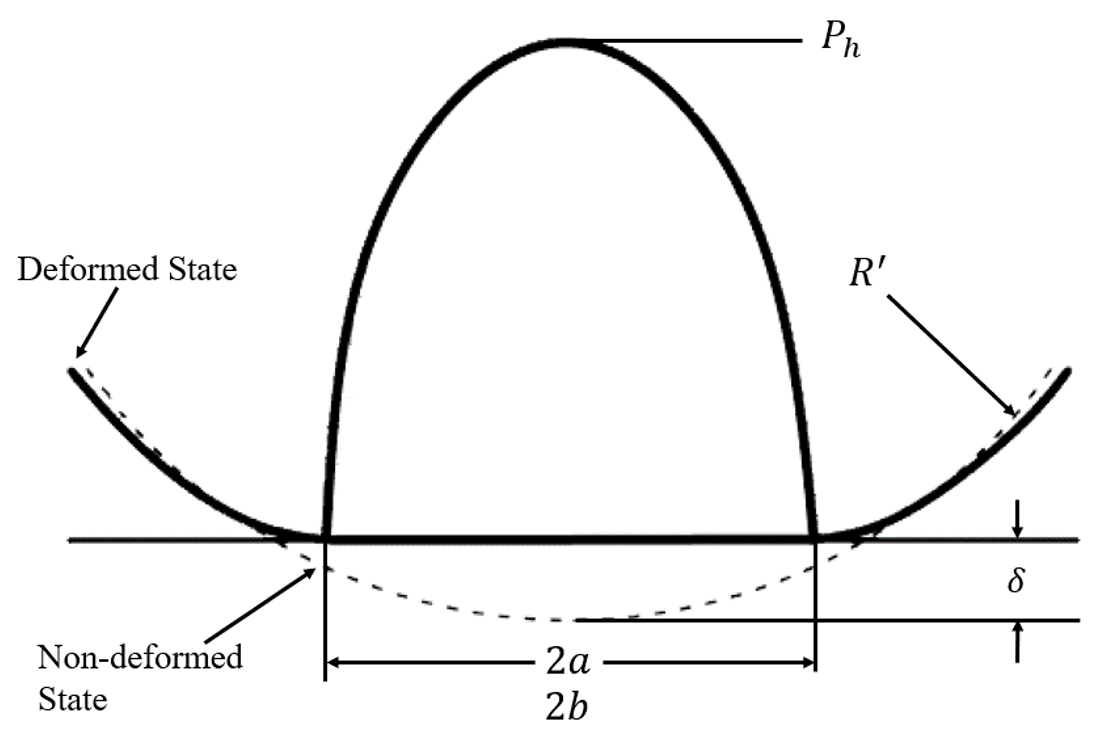
\includegraphics[width=100 mm]{Hertzian_Contact_Deflection.png}}
	\caption{Hertzian contact deflection.}
	\label{HertzianContactDeflection}
\end{figure}

The value of the deflection determines the stiffness of the contact and the displacement of the inner bearing race with respect to the outer. The contact area determines the contact pressures and hence maximum sub-surface stresses. Excessive sub-surface stress could lead to inelastic deformation and subsequent fatigue spalling.

Analytical formulae provide a way of calculating the dimensions of the contact patch, $b$, and the resultant maximum Hertzian pressure, $P_h$ given a known force, $w$, material properties and geometry of bodies. For the case of the line contact these are:

\begin{equation}\label{eq2.3}
	b=\sqrt{\frac{8 w R_{z x}}{\pi E_r}}
\end{equation}

\begin{equation}\label{eq2.4}
	P_h=\sqrt{\frac{2 w}{\pi b}}
\end{equation}

where $w$ is load per unit length.

\subsection{Line Contacts}

The contact between rolling elements and raceways and the subsequent load and deformation generated at this contact is regarded as one of the most important issues in rolling-element bearing modelling. For a ball bearing, classical Hertzian theory is used to calculate the load-deformation relationship. However, the line contact is more complex.

There exist three methods to determine this relationship for the line contact in roller bearings: the slicing technique, 3D contact method and the alternative slicing technique. The slicing technique \cite{Andreason1973} divides the roller-race contact region into a finite number of slices, with the total contact forces calculated from the summation of forces of each individual slice. Various formulae have been developed to perform this calculation, all yielding very similar results. A drawback of this method is that the load on each slice does not influence the surrounding slices as they are treated independently. This means that pressure concentrations such as edge stresses on the contact are not captured. The 3D contact method uses the Boussinesq half-space force-displacement relationships and flexibility method of structural analysis. The contact pressure distribution and normal approach between the bodies is found using an iterative scheme, making this a time-consuming method. Kabus et al. \cite{Kabus2012} addressed this in their 6-dof quasi-static time-domain bearing model  by pre-processing a series of contacts at different centreline approaches  and roller tilt angles, then interpolating these results in the actual simulations. This negated the need to solve the iterative scheme at each time step. This allowed for bearing misalignment, roller centrifugal forces, flange contact and roller tilt moments to be analysed. 

Teutsch and Sauer \cite{Teutsch2004} improved on the slicing technique with their alternative slicing method. Using a matrix of weighted influence coefficients, the effects of force on the deflection of neighbouring slices was captured. It is not too dissimilar in concept to the 3D contact method but with improved computation times. de Mul et al. \cite{DeMul1989_2} compared the slicing technique with their more complex non-Hertzian model and concluded that the simplicity and accuracy of the slicing method yielded accurate and faster results. Harris and Kotzalas \cite{Harris2007} also concluded that the slicing technique, whilst unable to reflect edge stress concentrations, provides a suitably accurate load-displacement result as stresses are only distributed over a small area. For the purpose of load equilibrium, these stresses can be neglected. Misalignment or loading on roller ends is not captured using this technique, therefore for fatigue life estimates this may produce non-conservative results; for this, the approach by Kabus et al. should be used. In general, the slicing technique is the most widely used, owing to its simplicity, speed, and sufficient accuracy.

\section{Elastohydrodynamic Lubrication}

\subsection{History}

Under the EHL regime, both the elastic deformation of the solids in contacts as well as hydrodynamic theory are considered. Elastic bodies in contact for the case of ellipsoidal contacts was first investigated by Hertz in 1881 \cite{Hertz1881}, allowing him to obtain the pressure distribution within an ellipsoidal contact. Separate studies on hydrodynamic lubrication were being performed by Reynolds in 1886 \cite{Reynolds1886}, based on a simplified version of the Navier-Stokes equation. It took a further 30 years before the two studies would be combined.

Early EHL studies began in 1916 when the pioneering work by Reynolds was applied to a simplified model of a gear-tooth contact by Martin \cite{Martin1916}; replicated as two contacting cylinders. This analysis assumed that the solid bodies were rigid and the lubricant to behave with constant viscosity (ie. a hydrodynamic analysis). The resultant pressures were too high and the film thickness so low (1-10~$nm$) that coverage of asperities (typical order of 100~$nm$ for machined gear teeth) was not possible. This contradicted experimental findings where machining tracks on high-speed gear tooth flanks were still visible after prolonged usage, which could only be explained by the presence of a sufficient lubricant film.

Between the 1930’s and 1950’s, significant research was performed to include both the elastic deformation of the surfaces and the effect of pressure on viscosity. Peppler \cite{Peppler1936} and Meldahl \cite{Meldahl1941} both included the effects of surface deformation for non-conformal contacts, with Gatcombe \cite{Gatcombe1945} amongst others investigating viscosity increase due to the high pressure in the contact area. Typical EHL pressures are in the range of 0.5-4~$GPa$ and the resulting piezo-viscous properties were found to be partially instrumental to forming the film.

Considered the origin of EHL, Grubin’s pioneering work in 1949 \cite{Grubin1949} combined both elastic deformation and viscosity increase under pressure in film thickness calculations for the first time. In this analysis, he assumed that the deformed surface profiles in a highly loaded lubricated contact matched those produced in a classic dry Hertzian contact of the same materials and loading conditions. Reynolds equation could then be solved at the inlet region of the contact and a more accurate determination of the separation of the solids in the central region was found. This led to a film thickness in the predicted range (an order higher than Martin’s theory) and a more realistic pressure distribution than previous work. This pioneering study formed the basis for future EHL studies.

The first numerical solution of the line contact problem was presented shortly after by Petrusevich \cite{Petrusovich1951} which agreed with Grubin’s main conclusions. It contained the three main features of an EHL contact: a nearly parallel film in the contact zone with local constriction at the exit, a Hertzian pressure profile, and secondary local maximum pressure or ‘spike’ at the outlet (see Figure \ref{EHL_Film_Pressure_Schematic}). In 1959, Dowson and Higginson \cite{Dowson1959} presented their numerical solution to the isothermal line contact EHL problem. Their iterative inverse method enabled the evaluation of film thickness and pressure distribution for line contact problems for lightly loaded cases. Throughout the 1960s, the authors investigated the effects of variables such as dimensionless surface velocity, materials parameter and load on EHL solutions. The authors then curve fitted their results and generated an empirical formula for isothermal line contacts \cite{Dowson1961}, which was then improved upon by Dowson \cite{Dowson1966} and Dowson and Toyoda \cite{Dowson1979}. The formulae predict the minimum film thickness as a function of the rolling velocity, load and material parameters.

Empirical formulae are widely used today for analytical calculations that do not require the computational intensity of a full numerical solution. They are, however, somewhat limited to the operating parameters used in original simulations and do not offer the capabilities of a full numerical solution, such as the modelling of inlet starvation at high speeds.

\subsection{Numerical Methods}

There are 2 main numerical methods for solving the elastohydrodynamic problem; direct and inverse. Typically, Reynolds equation is solved for pressure based on the lubricant film thickness. Early studies using this direct method suffered from convergence in highly loaded cases.

\paragraph{Inverse Method}

Ertel \cite{Ertel1939} introduced the inverse method for the hydrodynamic problem, which was adopted by Dowson and Higginson \cite{Dowson1959} for the EHL line contact problem. Here, the film thickness profile is found from a given pressure distribution. Solving the elastic deformation equation provides a second film thickness profile that corresponds to the same pressure distribution. This pressure distribution is then modified manually until the film thickness solutions converge.

This approach has some disadvantages. For low load cases with a non-parallel film shape in the contact region, this method is not suitable since the deviation of the Hertzian starting solution is too large. The film thickness equation is also insensitive to local variations in pressure. Finally, it is only suitable for line contact 1-dimensional cases since the Reynolds equation cannot be integrated for the two-dimensional case. Evans and Snidle \cite{Evans1982} overcame the 2-dimensional limitation by using their quasi-static solution where a direct method was applied at the inlet zone and the inverse method in the contact zone. The aim was to overcome the instabilities of the forward iterative method to solve heavily loaded contacts which were limited to 0.5 $GPa$, whereas common stresses in practice are typically in the order of 1.5 $GPa$, reaching as high as 4 $GPa$ in some cases. A solution was only found for heavily loaded cases and the approach was limited by the need for an accurate initial estimate for pressure.

\paragraph{Direct Method}

The direct iterative method is the most common method whereby Reynolds equation is solved to find the pressure with a given film thickness. This pressure distribution is used with the elastic equation to calculate a new film shape. The pressure distribution must also achieve equilibrium with the externally applied load.

Two different direct methods have been used to solve the discretized Reynolds equation. The first is the iterative technique which has been applied to the 1-dimensional line contact problem \cite{Hamrock1984} as well as the two-dimensional point \cite{Hamrock1976a} and elliptical \cite{Chittenden1985} contact problem. The Gauss-Seidel scheme was used, solving Reynolds equation for pressure based on film thickness and iterating between the two until convergence was met. Force equilibrium in an outer loop was calculated by integrating pressure across the contact domain and ensuring convergence between the resultant force and the applied external load. The solution comprises of 3 nested loops that must all converge. Under relaxation between successive iteration is applied to aid convergence, however this iterative method does not converge for high loads. Furthermore, the number of iterations to achieve convergence is large (ie. of the square of the number of computational points used) and thus excessive computation times result.

The second solution method is the Newton-Raphson method. This was first applied by Okumara \cite{Okumara1982} and later by Houpert and Hamrock \cite{Houpert1985}, where pressures as high as 4.8 $GPa$ were obtained with low CPU times. These low CPU times are a significant advantage of the Newton-Raphson methodology, with a smaller number of iterations resulting in much faster convergence than Gauss-Seidel.

Further numerical development came in the form of the multi-level method, first used by Lubrecht et al. in 1986 \cite{Lubrecht1986}. Venner et al. \cite{Venner1990} used a multilevel multi-integration for point and line contacts in 1990 to reduce the computational cost of solving the film thickness integral. This allowed more nodes in the computational domain to be used for more complex problems with again much faster solution times. Finer grids could therefore be used, yielding faster results than Newton-Raphson for more complex cases. The solution time was proportional to $n log(n)$, with $n $being the total number of nodes in the computational domain. This work was mainly focussed on reducing computational time for the point contact problem, with the authors acknowledging the applicability of the Newton-Raphson numerical scheme for the line contact problem.

\subsection{Starvation}

The assumption of a fully flooded inlet region to the contact is not always valid. Starvation may occur if insufficient lubricant is entrained into the contact; significantly affecting EHL characteristics such as film formation and friction coefficient. This starvation is found to be greater at higher speeds, with higher viscosity lubricants and limited lubricant supply \cite{Chevalier1995}. At high speeds, lubricant replenishment is diminished. For a fully flooded contact, the pressure builds upstream of the contact starting from a pressure gradient close to zero. With insufficient lubricant, the contacting bodies entrain two layers of lubricant, which then merge and form a meniscus at the contact inlet; causing the pressure rise to occur closer to the contact centre with a non-zero pressure gradient and reduced shape of the characteristic pressure distribution \cite{Lugt2011}.

Analytical work on this topic began for the line contact problem by Wolveridge et al. \cite{Wolveridge1970a} and later developed for the elliptical contact problem by Hamrock and Dowson \cite{Hamrock1976}. In these studies, the inlet distance to the centre of the contact domain is varied as an input parameter. As the inlet distance is extended, the flooded condition at the entrance to the contact becomes greater. At a certain inlet distance, the film thickness in the contact is hardly affected (see Figure \ref{Starvation_Hamrock_Dowson}), and this is defined as the threshold between starvation and a fully flooded inlet condition. For the case of shorter inlet distances and subsequent starved condition, an equation was presented that could adjust the starved film thickness based on the starvation level and flooded film thickness.

\begin{figure}
	\centerline{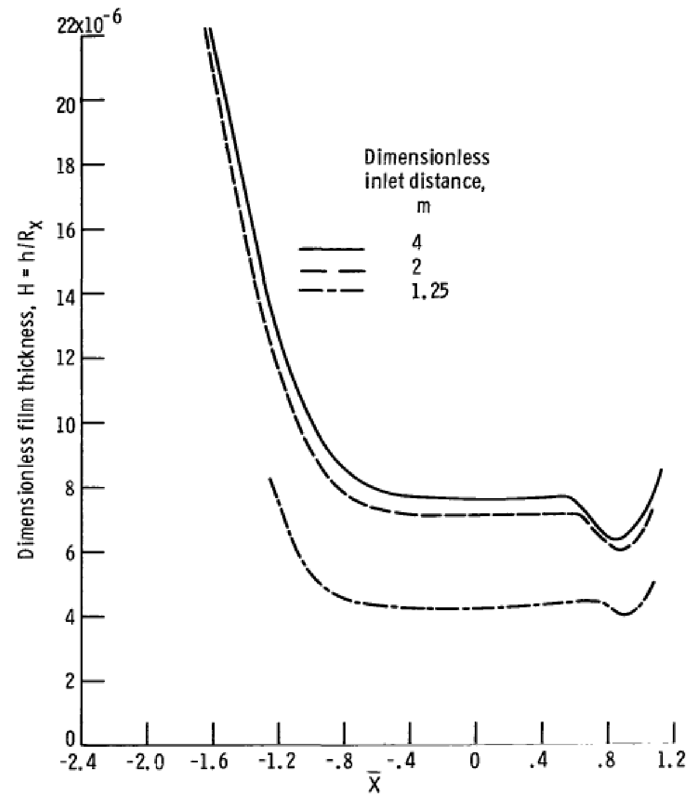
\includegraphics[width=90 mm]{Starvation_Hamrock_Dowson.png}}
	\caption [Effect of dimensionless inlet distance on film thickness for starvation modelling]{Effect of dimensionless inlet distance on film thickness for starvation modelling \cite{Hamrock1976}.}
	\label{Starvation_Hamrock_Dowson}
\end{figure}

\subsection{Thermal EHL}

Heat is generated in an EHL contact in two ways: due to the viscous shearing of the lubricant and the compressive action of the generated pressures \cite{Mohammadpour2015c}. Classic EHL theory is isothermal and considers a Newtonian fluid with no temperature rise from sliding at the conjunction. For the case of pure rolling, this is sufficient to predict film thickness and inlet temperature rise. Rolling element bearings, however, can undergo complex rolling and sliding motions depending on the nature of the loading and contact conditions. The presence of sliding requires a rheological model that considers the viscosity relationship with pressure as well as the use of the energy equation to calculate temperature rise within the lubricant film.

The three-dimensional energy equation has been solved by various authors for the line contact \cite{Yang2001}, point contact \cite{Kim1993},\cite{Kim1993a} and finite line contact \cite{Liu2002}. The generated heat is carried along the direction of entraining motion, in the direction of side leakage from the contact, and through the bounding surfaces of the contact. This can be reduced to fewer dimensions for the assumption of negligible heat transfer to the contacting bodies in the direction of the film thickness.

It has been found in the case of the point contact under low loads, thermal effects on pressure distribution and film thickness are negligible \cite{ZhuDong1984}. However, Kim and Sadeghi \cite{Kim1993} concluded that with higher loads, the temperature rise in the film is significant. Under pure rolling conditions, the lubricant film temperature rise was only a moderate 15~${ }^{\circ}\mathrm{C}$ above ambient and occurred at the inlet zone. As the slide/roll ratio was increased to 0.2, for the same load and speed conditions a temperature rise of 140~${ }^{\circ}\mathrm{C}$ above ambient resulted at the contact centre, with the dominant mode of heat transfer being shear heating in the contact. The authors also adjusted the ellipticity parameter of the contact \cite{Kim1993a}, with higher ellipticity parameters bringing the elliptical shape of the contact closer to that of a line. In this study, the load was more moderate, and the temperature rise for pure rolling and a slide/roll ratio of 0.2 was 4.5~${ }^{\circ}\mathrm{C}$ and 16~${ }^{\circ}\mathrm{C}$ respectively.

Habchi et al. \cite{Habchi2008} found that even under light loads and moderate speed conditions, thermal effects were still noticeable for Newtonian fluids. For lightly loaded cases, thermal and isothermal results were comparable up to entrainment velocities of 1~$m/s$ but began to diverge slightly above this: in line with experimental findings. Additionally, as the slide/roll ratio is increased above 0.5, both central and minimum films are found to decrease for the thermal model, whereas the isothermal model remains constant. This is due to shear heating reducing lubricant viscosity. The difference was found to be only 0.015 $\mu \mathrm{m}$ between pure rolling and close to pure sliding for a lightly loaded contact.

Shear thinning of the lubricant also occurs at the inlet region to the contact. EHL films are micron level thickness, and assuming a fully flooded inlet, not all of the lubricant will traverse into the contact. Rejected lubricant will then produce some reverse flows which will shear the lubricant, increasing the inlet temperature and hence reduce the viscosity of the fluid \cite{Stribeck1907}.

It is therefore clear that a thermal elastohydrodynamic model is necessary for highly loaded conditions with modest slide/roll ratios.

\subsection{Elastohydrodynamic Pressure and Film Characteristics}

If there is relative velocity between two lubricated contacting surfaces, a thin film is formed due to the wedge mechanism and lubricant is entrained into the contact. The pressure profile across the contact deviates from the dry Hertzian parabolic distribution due to the presence of the lubricant.

Figure \ref{EHL_Film_Pressure_Schematic} shows the deviation of the film pressure from the dry Hertzian pressure. The main deviation occurs at the outlet of the contact due to the exit conditions. At the entry of the contact, the increasing pressure profile acts to oppose the flow of lubricant into the contact due to the entraining motion. At the outlet, the Couette profile and the pressure differential acts in the same direction to force lubricant out of the contact. For mass flow rate of the lubricant across the contact to be conserved, an outlet constriction is formed to reduce the flow area. The pressure spike at the outlet generates this deformation of the surfaces to maintain this flow balance and is a result of the piezo-viscosity of the lubricant. The two laws that must be obeyed are therefore the force equilibrium (the differential of pressure across the contact must equal the applied force), and the flow continuity.

\begin{figure}
	\centerline{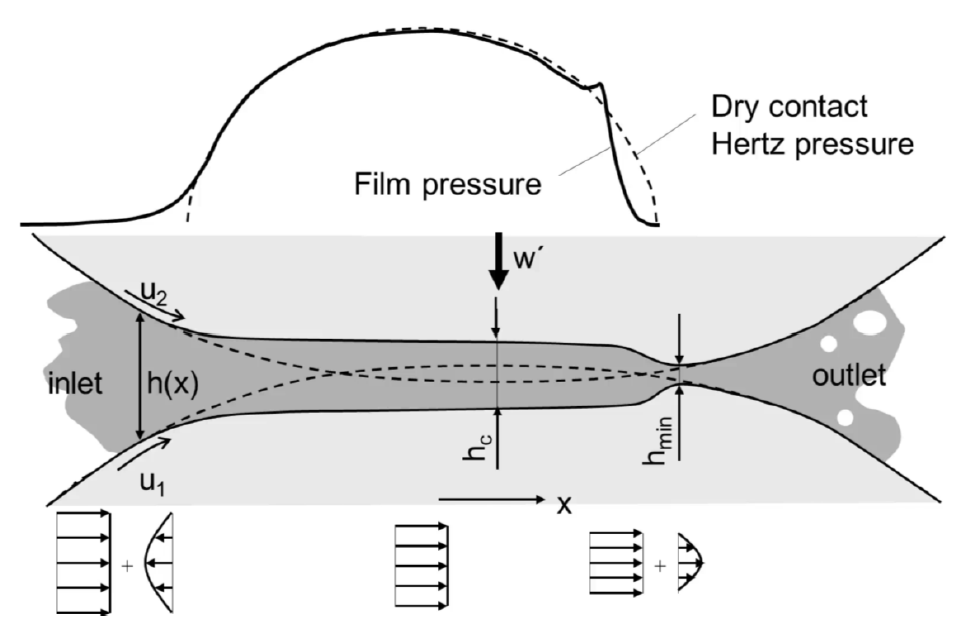
\includegraphics[width=125 mm]{EHL_Film_Pressure_Schematic.png}}
	\caption[EHL film and pressure distribution]{EHL film and pressure distribution \cite{Larsson2013}.}
	\label{EHL_Film_Pressure_Schematic}
\end{figure}

\subsection{Lubrication Regimes}

Lubricated contacts fall into four main regimes, these are:

\begin{itemize}
	\item \textbf{Hydrodynamic}: Contacting surfaces are completely separated by the lubricant film. Load is light, typically several Newtons. The contact surfaces do not experience deformation and resultant pressures are in the region of MPa.
	\item \textbf{Elastohydrodynamic}: Contacting surfaces are completely separated by lubricant film; however, load is medium to heavy. Contact deformation occurs and resultant contact pressures are in the region of GPa.
	\item \textbf{Mixed}: An interrupted oil film separates the two surfaces, ie. some asperity interaction occurs. Mixed lubrication can occur under any load and is dependent on the film thickness and asperity height.
	\item \textbf{Boundary}: The lubricant film is negligible, and surfaces directly interact. This a dry contact. At medium and high loads, Hertzian contact conditions can be assumed.
\end{itemize}

The loaded contact region of bearings are typically in the elastohydrodynamic regime of lubrication. The film thickness to asperity roughness height (lambda ratio) is large enough that the surface features do not typically influence the lubricant thickness and often a smooth surface is assumed. Under operation, emerging clearances result in unloaded regions of the bearing which can cause the roller-to-race contact to deviate from the elastohydrodynamic lubrication regime towards hydrodynamic regime, resulting in sliding and roller-cage collisions \cite{Mohammadpour2015c}. Hence, the contact may go through different regimes of lubrication throughout its rotation.

Film thickness and surface roughness are related by Stribeck \cite{Stribeck1907} using the specific film thickness:

\begin{equation}\label{eq2.5}
	\lambda_s=\frac{h}{\sigma}
\end{equation}
 
 where $h$ is the lubricant film thickness and $\sigma$ is the roughness height of the asperities on the contact surfaces. Figure \ref{Stribeck_Curve} presents the various lubrication regimes and their associated coefficient of friction. For rougher surfaces, mixed-EHL occurs where contact of surface asperities occurs, increasing friction. The coefficient of friction then reduces as the film increases or asperity height reduces, until the hydrodynamic regime is reached, and the thicker films increase viscous friction.

\begin{figure}
	\centerline{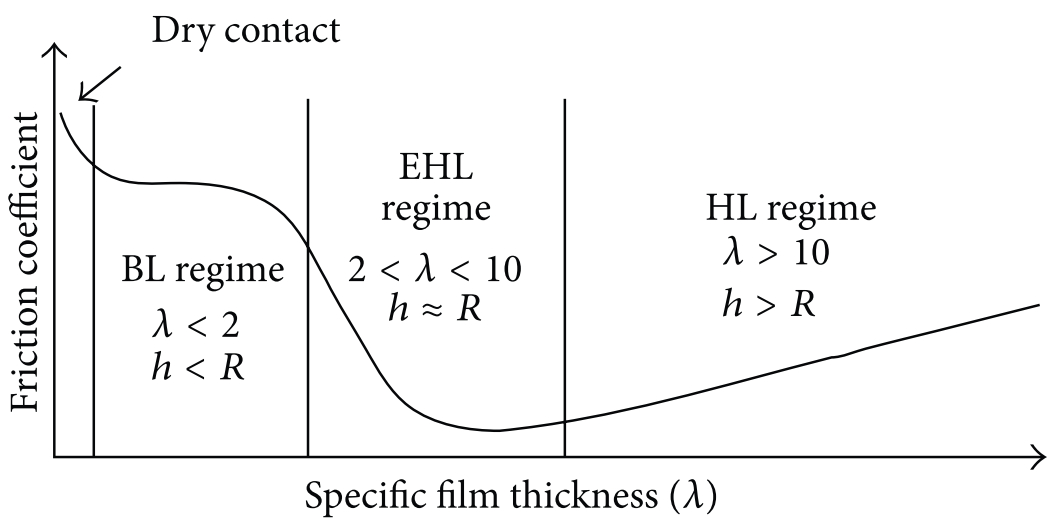
\includegraphics[width=100 mm]{Stribeck_Curve.png}}
	\caption[Stribeck curve and specific film thickness]{Stribeck curve and specific film thickness ($\lambda$) \cite{Ali2015}.}
	\label{Stribeck_Curve}
\end{figure}

\section{Artifical Neural Networks}

The most common ML algorithm used in tribological applications are ANNs. The first utilization of these were in the 1990s \cite{Argatov2019}. Ezugwu et al. implemented and ANN for wear rate and hence life predictions of ceramic cutting tools \cite{Ezugwu1995}. Their model had an 80\% success rate in predicting the failure mechanism of the tools. Rutherford et al. \cite{Rutherford1996} and Jones et al. \cite{Jones1997} developed on this success, focussing on wear rate predictions for coating materials and mechanical systems respectively. Jones et al. were able to achieve 90\% wear rate predication accuracy by optimising their ANN architecture using $R^2$ coefficients as a performance indicator. Similar studies were then conducted in the domain of friction and wear rate of composite materials \cite{Genel2003} \cite{Hayajneh2009} \cite{Zhang2002}, as well as tools steels \cite{Cavaleri2019}. 

Whilst the friction in the aforementioned studies was modelled under dry conditions, friction in lubricated contacts has also been modelled using ANNs. Bhaumik et al. \cite{Bhaumik2019a} used ANNs to develop a new lubricant with multiple friction modifiers (FM), considering load, speed and FM concentration as input variables, with the target output being coefficient of friction. A similar methodology was employed to develop biodegradable oils \cite{Bhaumik2019a}, validating both sets of studies using pin-on-disc friction measurements. Traction coefficients under various thermal-elastohydrodynamic operating conditions have also been investigated \cite{EchavarriOtero2014}, with the authors noting fast predictions of results with excellent accuracy (lower than 3\% error in most cases). Further lubricated studies involving relative viscosity predictions \cite{Afrand2016} \cite{HemmatEsfe2018} have achieved deviation margins of 1.5\% and 0.07\% respectively, substantially lower than empirical correlations.

Many further studies have been performed in the field of wear in manufacturing processes \cite{Ripa2004}. Previous studies had multiple input variables to the ANNs (speed, load, temperature, shear rate). For specific manufacturing processes with particular lubricant-surface combinations, the input data array can be drastically reduced to process-specific variables such as load, speed, and vibration. This approach was taken to investigate flank wear in drilling \cite{Panda2008} and surface roughness of machined parts \cite{Asilturk2011}. By reducing the number of input parameters, less training data was required to achieve good fits.

The studies referenced (\cite{Ezugwu1995} - \cite{Asilturk2011}) all shared a common approach of utilizing experimental data to train the ANNs. Whilst experimental data benefits from the lack of assumptions in numerical models, there is the limitation of high costs and time required for generating large datasets. Consequently, the training datasets for the ANN were limited to approximately one hundred points \cite{Zhang2002} \cite{Hayajneh2009}, or fewer \cite{Ezugwu1995} \cite{Rutherford1996}, with the largest (216 points) utilised by Cavaleri et al. \cite{Cavaleri2019}. Since the training process optimizes the ability of the ANN to interpolate between data points for varying input conditions, a greater number of training points is advantageous. It was noted by Ezugwu et al. \cite{Ezugwu1995} and Zhang et al. \cite{Zhang2002} that a significant improvement in ANN fit was achieved with a larger training data set. This is an observation shared across several studies and scientific applications \cite{Barbedo2018}.

An alternative method of achieving large data sets without the high financial and time cost of experimentation is to use numerical modelling. Wang et al. \cite{Wang2020} identified the need for larger training sets in the field of tribology. Their prediction for maximum Hertzian pressure in thermohydrodynamic contacts utilised a training data set that was generated using Reynolds equation. Whilst limited to the accuracy of the numerical model, the ANN benefits from much faster computation time. It crucially also allows for larger data sets to be generated that can cover a much larger range of input data; a requirement for implementation within dynamic models.

The Reynolds boundary value problem has also been solved using Physics Informed Neural Networks (PINN) by Almqvist \cite{Almqvist2021}. The study was not to improve on the numerical accuracy or efficiency of standard finite-difference based methods, rather to present an application of PINN in the field of tribology. Error analysis showed good agreement with the analytical solution, however further work is needed to improve the solving efficiency. Since the ANN is to be implicitly embedded within a dynamic simulation, efficiency is critical. Data driven solutions are therefore preferable. Marian et al. \cite{Marian2022} demonstrated for the first time the generation of EHL film thickness data using a Finite Element Method (FEM) to train an ANN. The ANNs could predict locally-resolved film thickness across the contact domain 25-times faster than FE-based EHL simulations.

Although ANNs lack the physical understanding provided by numerical solutions, they offer nearly real-time performance comparable to analytical solutions while benefiting from the accuracy of numerical methods \cite{EchavarriOtero2014}.

Echávarri et al. \cite{EchavarriOtero2014} comment on the "black box" nature of ANNs. Results from intermediate calculations are lost, which is often of interest for more in-depth analysis of contact condition; film thickness and pressure distributions and temperature for example. 

WHY DECIDED TO USE ANN - Look at study by Marian


It is now known that data-driven solutions, such as machine learning, can greatly enhance the computational efficiency of tribo-dynamic simulations without sacrificing accuracy. In this study, artificial neural networks (ANNs) were trained using numerical solutions constrained by lubrication regimes to ensure the quality of the training data set.

\section{Closure}
A review of the open literature shows that considerable advancements have been and continue to be made in the field of dynamic bearing modelling and tribology. However, there is a paucity of work integrating the two in the context of electrified automotive powertrains. The EHL film is shown to influence contact stiffness and hence dynamic behaviour at high entrainment velocities. With the trend towards high-speed motors in future automotive powertrains, this film growth must be considered. Furthermore, the investigation of this multi-physics interaction is constrained by the substantial computational effort required. The literature shows that ANNs can be successfully used to model tribological phenomena, suggesting that their integration into a dynamic model could provide an efficient and accurate solution.